%Master File:lectures.tex

\lesson{Wasserstein GANs}
\vspace{-1cm}
\begin{center}
  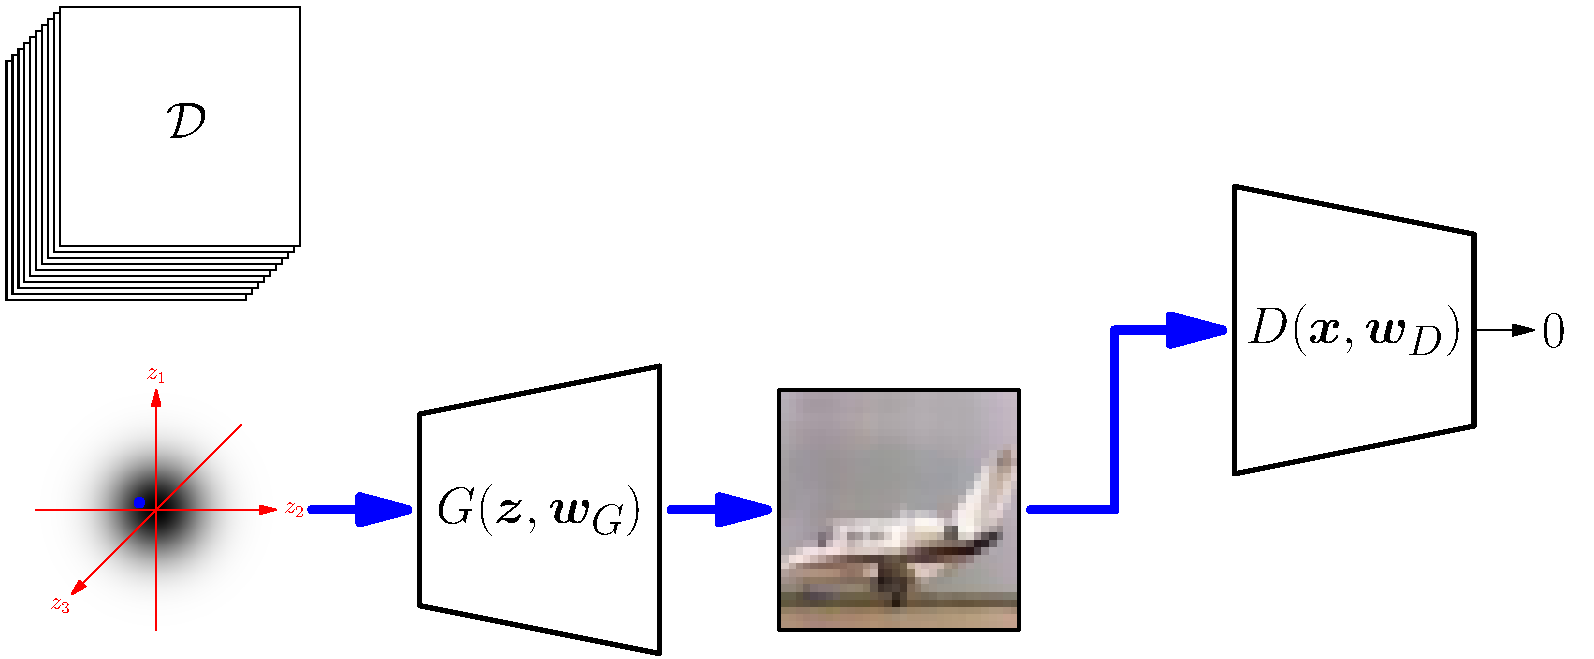
\includegraphics[width=0.9\linewidth]{gan-0}
\end{center}

\keywords{GANs, Wasserstein distance, Duality, WGANs}


%%%%%%%%%%%%%%%%%%%%%%% Next Slide %%%%%%%%%%%%%%%%%%%%%%%
\renewcommand{\Outline}{%
\begin{slide}
\section{Outline}

\begin{minipage}{8cm}\raggedright
  \begin{enumerate}
    \outlineitem{GANs}{gans}
    \outlineitem{Wasserstein Distance}{wasserstein}
    \outlineitem{Wasserstein GANs}{wgans}
  \end{enumerate}
\end{minipage}\hfill
\begin{minipage}{15cm}
  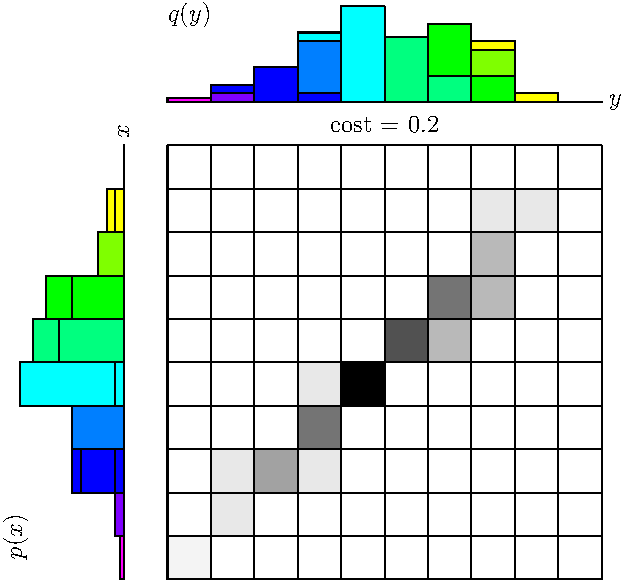
\includegraphics[width=15cm]{transportationCost-5}
\end{minipage}
\end{slide}
\addtocounter{outlineitem}{1}
}

\setcounter{outlineitem}{1}

%%%%%%%%%%%%%%%%%%%%%%% Next Slide %%%%%%%%%%%%%%%%%%%%%%%
\Outline % GANs
%%%%%%%%%%%%%%%%%%%%%%% Next Slide %%%%%%%%%%%%%%%%%%%%%%%

\begin{slide}
\section{Generative Adversarial Networks}

\begin{PauseHighLight}
  \begin{itemize}
  \item One of the applications of Deep Learning that has most excited
    the public are \emph{Generative Adversarial Networks} or GANs\pause
  \item Their aim is to generate new random samples from the same
    distribution as some training set, $\mathcal{D}$\pause
  \item Their number of real world applications are\pause{}
    questionable\pauseb
  \item But nobody cares because they are cool!\pauseb 
  \item \textit{Out of date warning:} someone invented diffusion
    models\pauseb
  \end{itemize}
\end{PauseHighLight}


\end{slide}

%%%%%%%%%%%%%%%%%%%%%%% Next Slide %%%%%%%%%%%%%%%%%%%%%%%

\begin{slide}
\section{How GANs Work}

\pb\pause\pauselevel{=1}
\begin{center}
  \multipdf[width=\linewidth]{gan}\pause
\end{center}
\end{slide}

%%%%%%%%%%%%%%%%%%%%%%% Next Slide %%%%%%%%%%%%%%%%%%%%%%%

\begin{slide}
\section{Training GANs}

\begin{PauseHighLight}
  \begin{itemize}
  \item The loss of the generator depends on its ability to trick the
    discriminator\pause
  \item The loss of the discriminator depends on its ability not to be
    tricked\pause
  \item We try to train the two networks simultaneously\pause
  \item We hope that over time the generator produces better and
    better fakes\pause
  \end{itemize}
\end{PauseHighLight}

\end{slide}
%%%%%%%%%%%%%%%%%%%%%%% Next Slide %%%%%%%%%%%%%%%%%%%%%%%

\begin{slide}
\section{Problems of GANs}

\begin{PauseHighLight}
  \begin{itemize}
  \item GANs are notoriously difficult to train\pause
  \item The generator and discriminator training can decouple\pause
  \item Often the discriminator becomes too good at correctly
    identifying the generated images\pause
  \item Then there can be little gradient information to help the
    generator as every small change in parameters doesn't significantly
    change the discriminator decision\pause
  \item To try to solve this problem we first make a seemly
    unconnected diversion\pause
  \end{itemize}
\end{PauseHighLight}
\end{slide}

%%%%%%%%%%%%%%%%%%%%%%% Next Slide %%%%%%%%%%%%%%%%%%%%%%%
\Outline % Wasserstein Distance
%%%%%%%%%%%%%%%%%%%%%%% Next Slide %%%%%%%%%%%%%%%%%%%%%%%

\begin{slide}
\section{Measuring Distances Between Distributions}

\begin{PauseHighLight}
  \begin{itemize}
  \item In many machine learning tasks we want to minimise the
    distance between two probability distributions\pause
  \item This requires that we can measure distances between
    probability distributions\pause
  \item One prominent measure is the Kullback-Leibler or KL divergence
    \begin{align*}
      \mathrm{KL}(p\|q) = \int p(\bm{x}) \,
      \logg{\frac{p(\bm{x})}{q(\bm{y})}} \, \dd \bm{x}\pause
    \end{align*}
  \item This is very commonly used in ML (e.g. VAEs, Variational
    Approximation)\pause
  \end{itemize}
\end{PauseHighLight}

\end{slide}

%%%%%%%%%%%%%%%%%%%%%%% Next Slide %%%%%%%%%%%%%%%%%%%%%%%

\begin{slide}
\section[-2]{Trouble with KL}

\begin{PauseHighLight}
  \begin{itemize}
  \item KL-divergences are non-negative quantities that are minimised
    when the two probability distributions are the same\pause
  \item They are not distances (they aren't symmetric and they don't
    satisfy the triangular inequality)\pause
  \item
    \begin{rightImage}{divergentKL}
      We don't really care about this, but what we do care about is
    that if $q(\bm{x})=0$ when $p(\bm{x})\neq 0$ then
    $\logg{\frac{p(\bm{x})}{q(\bm{y})}}$ diverges\pause
    \end{rightImage}
  \item We can therefore have distributes that seem very similar but
    their KL-divergence is huge (or infinite)\pause
  \end{itemize}
\end{PauseHighLight}

\end{slide}

%%%%%%%%%%%%%%%%%%%%%%% Next Slide %%%%%%%%%%%%%%%%%%%%%%%

\begin{slide}
\section[-1]{Wasserstein Distance}

\begin{PauseHighLight}
  \begin{itemize}
  \item A more benign measure of the differences between two
    probability functions is the \emph{Wasserstein} or \emph{Earth
      Moving} distance\pause
  \item
    \begin{rightImage}{divergentKL}
    This is a true distance, but more importantly for us it
    measure distance in a very natural way so that distributions that
    are close has a small Wasserstein distance\pause
    \end{rightImage}
  \item Although this seems contrived if our probability distribution
    represents the probability of a $128\times128$ matrix of real
    valued triples represents an image of dog, then it is easy to
    imagine that the Wasserstein distance may be more benign than the
    KL-divergence\pause
  \end{itemize}
\end{PauseHighLight}

\end{slide}
%%%%%%%%%%%%%%%%%%%%%%% Next Slide %%%%%%%%%%%%%%%%%%%%%%%

\begin{slide}
\section[-2]{High Probability Manifold}

\begin{center}
  \makebox(100,170)[c]{\includegraphics[width=0.7\linewidth]{manifold}}
\end{center}
\end{slide}

%%%%%%%%%%%%%%%%%%%%%%% Next Slide %%%%%%%%%%%%%%%%%%%%%%%

\begin{slide}
\section{Transportion Policy}

\begin{PauseHighLight}
  \begin{itemize}
  \item But how do we formalise the Wasserstein distance?\pause
  \item A good place to start is to define a transportation policy
    $\gamma(\bm{x},\bm{y})$ with
    \begin{align*}
      \int \gamma(\bm{x},\bm{y}) \, \dd \bm{y} &= p(\bm{x}) &
      \int \gamma(\bm{x},\bm{y}) \, \dd \bm{x} &= q(\bm{y})\pause
    \end{align*}
  \item This looks like a joint probability distribution, but we
    interpret $\gamma(\bm{x},\bm{y})$ as the amount of probability
    mass/density that we transfer from $p(\bm{x})$ to $q(\bm{y})$\pause
  \end{itemize}
\end{PauseHighLight}

\end{slide}

%%%%%%%%%%%%%%%%%%%%%%% Next Slide %%%%%%%%%%%%%%%%%%%%%%%

\begin{slide}
\section[-2]{Transportation Policy}

\pb
\pause\pauselevel{=1}
\begin{center}
  \multipdf[width=0.65\linewidth]{transportationPolicy}\pause
\end{center}
\end{slide}

%%%%%%%%%%%%%%%%%%%%%%% Next Slide %%%%%%%%%%%%%%%%%%%%%%%

\begin{slide}
\section{The Cost of Transport}

\begin{PauseHighLight}
  \begin{itemize}
  \item We want to choose the transportation policy that minimises the
    amount of probability mass we need to move\pause
  \item Let $d(\bm{x},\bm{y})=\|\bm{x}-\bm{y}\|$ be a distance measure
    then the cost of a transportation policy is
    \begin{align*}
      C(\gamma) = \int \int d(\bm{x},\bm{y})\,\gamma(\bm{x},\bm{y}) \,
      \dd\bm{x}\,\dd\bm{y}\pause = \av[\gamma]{d(\bm{x},\bm{y})}
    \end{align*}
    where we interpret $\gamma(\bm{x},\bm{y})$ as a probability
    distribution\pauseb
  \item Usually we take $d(\bm{x},\bm{y})$ to be the Euclidean
    distance, but we can choose any distance\pause
  \end{itemize}
\end{PauseHighLight}

\end{slide}

%%%%%%%%%%%%%%%%%%%%%%% Next Slide %%%%%%%%%%%%%%%%%%%%%%%

\begin{slide}
\section[-2]{Transportation Cost}

\pb
\pause\pauselevel{=1}
\begin{center}
  \multipdf[width=0.65\linewidth]{transportationCost}\pause
\end{center}
\end{slide}


%%%%%%%%%%%%%%%%%%%%%%% Next Slide %%%%%%%%%%%%%%%%%%%%%%%

\begin{slide}
\section{The Wasserstein Distance}

\begin{PauseHighLight}
  \begin{itemize}
  \item The Wasserstein distance $W(p,q)$ between two probability
    distributions is defined as
    \begin{align*}
      W(p,q) = \min_{\gamma \in \Lambda(p,q)}
      \av[\gamma]{d(\bm{x},\bm{y})}\pause
    \end{align*}
  \item Where $\Lambda(p,q)$ is the set of joint distributions
    $\gamma(\bm{x},\bm{y})$ such that
    \begin{align*}
      \int \gamma(\bm{x},\bm{y}) \, \dd \bm{y} &= p(\bm{x}) &
      \int \gamma(\bm{x},\bm{y}) \, \dd \bm{x} &= q(\bm{y})\pause
    \end{align*}
  \end{itemize}
\end{PauseHighLight}

\end{slide}

%%%%%%%%%%%%%%%%%%%%%%% Next Slide %%%%%%%%%%%%%%%%%%%%%%%

\begin{slide}
\section[-1]{Computing the Wasserstein Distance}

\begin{PauseHighLight}
  \begin{itemize}
  \item To compute the Wasserstein distance we have to solve a
    minimisation task!\pause
  \item This looks nasty, but it is a (continuous) linear programmming
    problem\pause
  \item Suppose $p$ and $q$ were discrete distribution (i.e. $\bm{x}$
    and $\bm{y}$ only take discrete points)\pause
  \item Then we could treat each value of $\gamma(\bm{x},\bm{y})$ as
    an element of a vector $\bm{\gamma}$ and each value of
    $d(\bm{x},\bm{y})$ as an element of a vector $\bm{D}$\pause
  \item Our objective is to choose $\bm{\gamma}$ to minimise
    $\bm{D}^\tr\bm{\gamma}$\pause
  \end{itemize}
\end{PauseHighLight}

\end{slide}

%%%%%%%%%%%%%%%%%%%%%%% Next Slide %%%%%%%%%%%%%%%%%%%%%%%

\begin{slide}
\section[-3]{Constraints}
  
\begin{PauseHighLight}
  {\small
\begin{align*}
  \sum_j \gamma(\bm{x}_i,\bm{y}_j) &= p(\bm{x}_i) &
 \sum_i \gamma(\bm{x}_i,\bm{y}_j) &= q(\bm{y}_j)
\end{align*}}
\begin{center}
  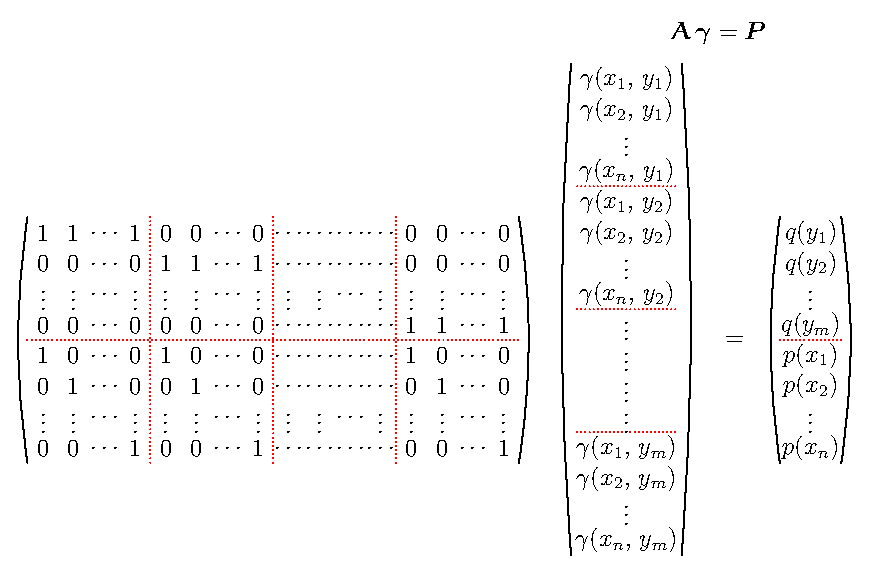
\includegraphics[width=0.8\linewidth]{Amat}\pause
\end{center}
\end{PauseHighLight}

\end{slide}

%%%%%%%%%%%%%%%%%%%%%%% Next Slide %%%%%%%%%%%%%%%%%%%%%%%

\begin{slide}
\section[-2]{Lagrange Formulation}

\begin{PauseHighLight}
  \begin{itemize}
  \item For discrete distributions
    \begin{align*}
      \min_{\bm{\gamma}} \bm{D}^\tr \mat{\gamma} \hspace{5cm} \\
      \text{subject to} \quad
      \mat{A}\,\bm{\gamma} = \bm{P}, \quad \bm{\gamma} \geq 0\pause
    \end{align*}
  \item Writing the Lagrangian 
    \begin{align*}
      \mathcal{L}(\bm{\gamma},\bm{\alpha})
      = \bm{D}^\tr \bm{\gamma} - \bm{\alpha}^\tr \left(
      \mat{A}^\tr \bm{\gamma} - \bm{P}\right)
    \end{align*}
    where $\bm{\alpha}$ is a vector of Lagrange multipliers\pause
  \item The solution to the discrete optimisation problem is given by
    \begin{align*}
      \min_{\bm{\gamma}} \, \, \max_{\bm{\alpha}} \,
      \mathcal{L}(\bm{\gamma},\bm{\alpha}) \pause
    \end{align*}
  \end{itemize}
\end{PauseHighLight}

\end{slide}

%%%%%%%%%%%%%%%%%%%%%%% Next Slide %%%%%%%%%%%%%%%%%%%%%%%

\begin{slide}
\section{Dual Form}

\begin{PauseHighLight}
  \begin{itemize}
  \item We can rearrange
    \begin{align*}
      \mathcal{L}(\bm{\gamma},\bm{\alpha})
      &= \bm{D}^\tr \bm{\gamma} - \bm{\alpha}^\tr \left(
        \mat{A} \bm{\gamma} - \bm{P}\right)\pause \\
      &= \bm{P}^\tr \bm{\alpha} - \bm{\gamma}^\tr \left(
        \mat{A}^\tr \bm{\alpha} - \bm{D}\right)\pause
    \end{align*}
  \item We note that $\bm{\gamma}\geq 0$ so the dual problem is to
    find a vector $\bm{\alpha}$ that maximises $\bm{P}^\tr
    \bm{\alpha}$ subject to the constraints $\mat{A}^\tr \bm{\alpha}
    \leq \bm{D}$\pause
  \item Although the vector form allows us to make connections with
    our earlier discussion of linear programming, it is a little
    difficult to interpret\pause
  \end{itemize}
\end{PauseHighLight}

\end{slide}

%%%%%%%%%%%%%%%%%%%%%%% Next Slide %%%%%%%%%%%%%%%%%%%%%%%

\begin{slide}
  \section{Explicit Form}


\begin{PauseHighLight}
  \begin{itemize}\footnotesize
  \item We can write a Lagrangian for the original problem
    \begin{align*}
      \mathcal{L} = \sum_{i,j} d(\bm{x}_i,\bm{y}_i)
      \gamma(\bm{x}_i,\bm{y}_j)
      &- \sum_i \alpha(\bm{x}_i) \left( \sum_j \gamma(\bm{x}_i,\bm{y}_j) -p(\bm{x}_i)\right)\\
      &- \sum_j \beta(\bm{y}_j) \left( \sum_i \gamma(\bm{x}_i,\bm{y}_j) -q(\bm{y}_j)\right)
    \end{align*}
    subject to $\gamma(\bm{x}_i,\bm{y}_j)\geq 0$\pause{} where $\alpha(\bm{x}_i)$ and $\beta(\bm{y}_j)$
    are Lagrange multipliers (they are components of $\bm{\alpha}$)\pauseb
  \item Rearranging
    \begin{align*}
      \mathcal{L} = \sum_i \alpha(\bm{x}_i)\,p(\bm{x}_i) + \sum_j \beta(\bm{y}_j)\,q(\bm{y}_j)
      -\sum_{i,j} \gamma(\bm{x}_i,\bm{y}_j)\left( \alpha(\bm{x}_i) + \beta(\bm{y}_j) -
      d(\bm{x}_i,\bm{y_i})\right)\pause
    \end{align*}
  \item This is eqivalent to maximising $\sum_i \alpha(\bm{x}_i)\,p(\bm{x}_i) +
    \sum_j \beta(\bm{y}_j)\,q(\bm{y}_j)$, subject to
    \begin{align*}
      \forall i,j \quad \alpha(\bm{x}_i) + \beta(\bm{y}_j) \leq d(\bm{x}_i,\bm{y_j})\pause
    \end{align*}
  \end{itemize}
\end{PauseHighLight}

\end{slide}


%%%%%%%%%%%%%%%%%%%%%%% Next Slide %%%%%%%%%%%%%%%%%%%%%%%

\begin{slide}
  \section{Continuous Form}


\begin{PauseHighLight}
  \begin{itemize}\footnotesize
  \item We can write a Lagrangian for the continuous problem
    \begin{align*}
      \mathcal{L} = \iint d(\bm{x},\bm{y})\, \gamma(\bm{x},\bm{y})
      \, \dd \bm{x}\,\dd \bm{y}
      &- \int \alpha(\bm{x}) \left( \int \gamma(\bm{x},\bm{y})\,\dd \bm{y}
        - p(\bm{x})\right) \, \dd \bm{x}\\
      &- \int \beta(\bm{y}) \left( \int \gamma(\bm{x},\bm{y}) \, \dd
        \bm{x} -q(\bm{y})\right) \, \dd \bm{y}
    \end{align*}
    subject to $\gamma(\bm{x},\bm{y})\geq 0$\pause{} where
    $\alpha(\bm{x})$ and $\beta(\bm{y})$ are Lagrange multiplier
    functions\pauseb
  \item Rearranging
    \begin{align*}
      \mathcal{L} = \int \alpha(\bm{x})\,p(\bm{x})\, \dd \bm{x}
      + \int \beta(\bm{y})\,q(\bm{y})\,\dd \bm{y}
      -\iint \gamma(\bm{x},\bm{y})\left( \alpha(\bm{x}) + \beta(\bm{y}) -
      d(\bm{x},\bm{y})\right)\, \dd \bm{x}\,\dd \bm{y}\pause
    \end{align*}
  \item This is eqivalent to maximising
    $\int \alpha(\bm{x})\,p(\bm{x})\, \dd \bm{x} + \int
    \beta(\bm{y})\,q(\bm{y})\,\dd \bm{y}$, subject to
    \begin{align*}
      \alpha(\bm{x}) + \beta(\bm{y}) \leq d(\bm{x},\bm{y})\pause
    \end{align*}
  \end{itemize}
\end{PauseHighLight}

\end{slide}

%%%%%%%%%%%%%%%%%%%%%%% Next Slide %%%%%%%%%%%%%%%%%%%%%%%

\begin{slide}
\section{Dual Form Constraint}

\begin{PauseHighLight}
  \begin{itemize}
  \item We note that $\alpha(\bm{x}) + \beta(\bm{y}) \leq d(\bm{x},\bm{y})$ for
    all $\bm{x}$ and $\bm{y}$\pause
  \item This has to be true when $\bm{x}=\bm{y}$ so that
    \begin{align*}
      \alpha(\bm{x}) + \beta(\bm{x}) \leq d(\bm{x},\bm{x}) = 0\pause
    \end{align*}
  \item So $\beta(\bm{x}) = -\alpha(\bm{x}) - \epsilon(\bm{x})$ where
    $\epsilon(\bm{x})\geq0$\pause
  \item But want to maximise {\small
    \begin{align*}
      \int \alpha(\bm{x})\,p(\bm{x})\, \dd \bm{x} + \int
      \beta(\bm{y})\,q(\bm{y})\,\dd \bm{y}
      = \int \alpha(\bm{x})\,\left(p(\bm{x}) - q(\bm{x})\right) \, \dd
      \bm{x} - \int q(\bm{x}) \, \epsilon(\bm{x}) \,\dd\bm{x} \pause
    \end{align*}}
  \item This is maximised when $\epsilon(\bm{x})=0$\pause{}
    i.e. $\beta(\bm{x}) = - \alpha(\bm{x})$\pauseb
  \end{itemize}
\end{PauseHighLight}

\end{slide}

%%%%%%%%%%%%%%%%%%%%%%% Next Slide %%%%%%%%%%%%%%%%%%%%%%%

\begin{slide}
\section{Dual Form}

\begin{PauseHighLight}
  \begin{itemize}
  \item Thus the dual problem is to find a function $\alpha(\bm{x})$---or a
    vector of functions $(\alpha(\bm{x}_i)|i)$---that maximises
    \begin{align*}
      \int \alpha(\bm{x})\,\left(p(\bm{x}) - q(\bm{x})\right) \, \dd \bm{x}
    \end{align*}
  \item Subject to the constraint
    \begin{align*}
      \alpha(\bm{x}) - \alpha(\bm{y}) \leq d(\bm{x},\bm{y}) = \| \bm{x}-\bm{y} \|\pause
    \end{align*}
  \item This is a continuity constraint on the Lagrange multiplier
    function $\alpha(\bm{x})$ known as Lipschitz-1\pause
  \end{itemize}
\end{PauseHighLight}

\end{slide}

%%%%%%%%%%%%%%%%%%%%%%% Next Slide %%%%%%%%%%%%%%%%%%%%%%%

\begin{slide}
\section[-2]{Lipschitz-1 Functions}

\begin{PauseHighLight}
  \begin{itemize}
  \item We note for a Lipschitz-1 function and any unit vector $\bm{u}$
    \begin{align*}
      \bm{u}^\tr\grad \alpha(\bm{x}) = \lim_{\epsilon \rightarrow 0}
      \frac{\alpha(\bm{x})-\alpha(\bm{x}+\epsilon \,
      \bm{u})}{\epsilon} \pause
      \leq \frac{\epsilon}{\epsilon} = 1 \pauseb
    \end{align*}
  \item That is, at every point the gradient in all directions must be
    less than 1\pause{} (since the gradient defines the direction of greatest
    increase it is both necessary and sufficient for $\|\grad
    \alpha(\bm{x})\|\leq1$ everywhere)\pauseb
  \end{itemize}
  \begin{center}
    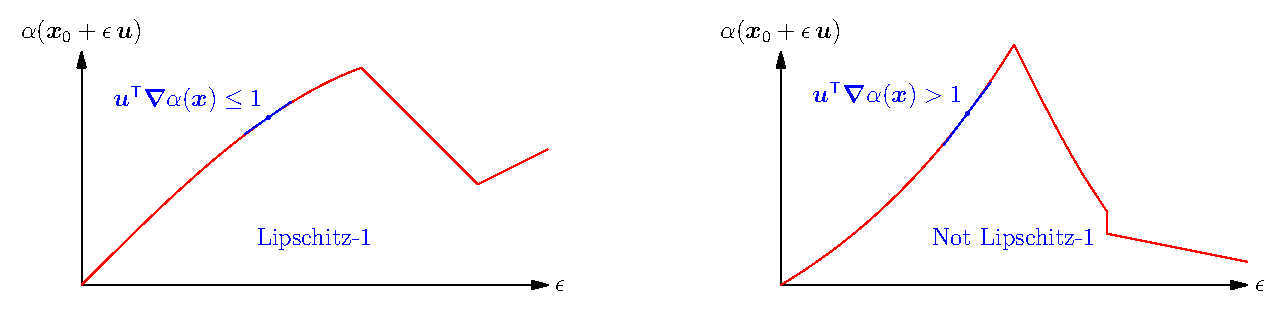
\includegraphics[width=\linewidth]{Lipschitz1}\pause
  \end{center}
\end{PauseHighLight}
  

\end{slide}


%%%%%%%%%%%%%%%%%%%%%%% Next Slide %%%%%%%%%%%%%%%%%%%%%%%

\begin{slide}
\section[-2]{Calculating the Wasserstein Distance}

\begin{PauseHighLight}
  \begin{itemize}
  \item To recall the big picture we want to compute the Wasserstein
    distance
    \begin{align*}
       W(p,q) = \min_{\gamma \in \Lambda(p,q)}
      \av[\gamma]{d(\bm{x},\bm{y})}\pause
    \end{align*}
  \item For high dimensional objects $\gamma(\bm{x},\bm{y})$ would be
    a huge object to approximate\pause
  \item Instead we can compute the Wasserstein distance in the dual
    formulation
    \begin{align*}
      \hspace*{-1em}W(p,q) = \max_{\alpha(\bm{x})} \int \alpha(\bm{x})\,\left(p(\bm{x}) -
      q(\bm{x})\right) \, \dd \bm{x} \pause
      = \max_{\alpha} \av[p]{\alpha(\bm{X})} - \av[q]{\alpha(\bm{X})}\pauseb
    \end{align*}
    subject to the constraint that $\alpha(\bm{x})$ is a Lipschitz-1
    function\pause
  \end{itemize}
\end{PauseHighLight}

\end{slide}


%%%%%%%%%%%%%%%%%%%%%%% Next Slide %%%%%%%%%%%%%%%%%%%%%%%
\Outline % WGANs
%%%%%%%%%%%%%%%%%%%%%%% Next Slide %%%%%%%%%%%%%%%%%%%%%%%

\begin{slide}
\section{Back to GANs}

\begin{PauseHighLight}
  \begin{itemize}
  \item What has this got do with GANs?\pause
  \item Suppose we want to minimise the distance between the
    distribution $p(\bm{x})$ of real images (of which $\mathcal{D}$
    are samples) and the distribution $q(\bm{x})$ of images drawn from
    a generator\pause
  \item We can use a normal GAN generator, $G(\bm{z}, \bm{w}_G)$, that
    generates an image when given a random variable
    $\bm{z}\sim\mathcal{N}(\bm{0},\mat{I})$\pause 
  \item To do this we choose the weights, $\bm{w}_G$ of the generator
    to minimise
    \begin{align*}
      W(p,q) = \max_{\alpha(\bm{x})} \left( \av[\bm{x}\sim p]{\alpha(\bm{x})} -
      \av[\bm{x}\sim q]{\alpha(\bm{x})} \right)\pause 
    \end{align*}
  \end{itemize}
\end{PauseHighLight}

\end{slide}

%%%%%%%%%%%%%%%%%%%%%%% Next Slide %%%%%%%%%%%%%%%%%%%%%%%

\begin{slide}
\section{Estimating Expectations}

\begin{PauseHighLight}
  \begin{itemize}
  \item Although we can't compute $\av[p]{\alpha(\bm{x})}$ and
    $\av[q]{\alpha(\bm{x})}$ exactly, we can estimate them from
    samples
    \begin{align*}
     \av[p]{\alpha(\bm{x})}
      &\approx \frac{1}{|\mathcal{B}|}
        \sum_{\bm{x}\in\mathcal{B}} \alpha(\bm{x}),
      &
        \av[q]{\alpha(\bm{x})}
      &\approx \frac{1}{n} \sum_{i=1}^n
        \alpha(G(\bm{z}_i,\bm{w}_G))\pause
    \end{align*}
  \item where $\mathcal{B}\subset\mathcal{D}$ is a minibatch of true
    images and $\bm{z}_i\sim\mathcal{N}(\bm{0},\mat{I})$\pause
  \item From this we can choose $\bm{w}_G$ to minimise
    \begin{align*}
      C = \frac{1}{|\mathcal{B}|}
      \sum_{\bm{x}\in\mathcal{B}} \alpha(\bm{x}) -
      \frac{1}{n} \sum_{i=1}^n \alpha(G(\bm{z}_i,\bm{w}_G))\pause
    \end{align*}
  \end{itemize}
\end{PauseHighLight}
\end{slide}

%%%%%%%%%%%%%%%%%%%%%%% Next Slide %%%%%%%%%%%%%%%%%%%%%%%

\begin{slide}
\section{The Critic}

\begin{PauseHighLight}
  \begin{itemize}
  \item For this quantity to approximate the Wasserstein distance we
    need to find a function $\alpha(\bm{x},\bm{w}_\alpha)$ that
    maximises $C$\pause
  \item To do this we learn a second network, the critic or
    discriminator whose job it is to maximise
    \begin{align*}
      C = \frac{1}{|\mathcal{B}|} \sum_{\bm{x}\in\mathcal{B}} \alpha(\bm{x},\bm{w}_\alpha) -
      \frac{1}{n} \sum_{i=1}^n \alpha(G(\bm{z}_i,\bm{w}_G),\bm{w}_\alpha)\pause
    \end{align*}
  \item The network $\alpha(\bm{x},\bm{w}_\alpha)$ should be
    Lipschitz-1 (which we usually botched by, for example, by setting
    the spectral norm of the convolutional weight matrix to 1)\pause
  \end{itemize}
\end{PauseHighLight}

\end{slide}


%%%%%%%%%%%%%%%%%%%%%%% Next Slide %%%%%%%%%%%%%%%%%%%%%%%

\begin{slide}
\section{Wasserstein GANs}

\pb\pause\pauselevel{=1}
\begin{center}
  \multipdf[width=\linewidth]{wgan}\pause
\end{center}
\end{slide}


%%%%%%%%%%%%%%%%%%%%%%% Next Slide %%%%%%%%%%%%%%%%%%%%%%%

\begin{slide}
\section{Lesson}

\begin{PauseHighLight}
  \begin{itemize}
  \item Wasserstein GANs are, at least for me, one of the most elegant
    pieces of theory in recent years\pause
  \item By trying to minimise the Wasserstein distance between the
    distribution of a generator and a true distribution we arrive at
    optimising two adversarial networks just like a GAN\pause
  \item This uses a rather beautiful dual formulation\pause
  \item It is claimed that W-GANs solve many of the problems of
    traditional GANs\pause
  \end{itemize}
\end{PauseHighLight}

\end{slide}





%%% Local Variables:
%%% TeX-master: "lectures"
%%% End:
